%----------------------------------------------------------------------
\section{Future Work}
%----------------------------------------------------------------------
To conclude, our proposed system was proved to be a feasible solution to achieve efficient OLAP queries processing on large graph datasets. We summarize future work as follows. First, as reflected in experiment results \ref{Results and Discussion}, efficiency performance of our system is affected by system settings, hence study on appriopriate system settings would be a valuable followup for our work. Second, the system we implemented so far supports SPARQL like queries over schema graph, instead of data graph. It is realizable to enable processing SPARQL like queries over data graph within our proposed solution framework. The key issue is take isomorphism into consideration during query decomposition and composition. Last but not least, greedy selection framework is with no doubt not a perfect solution for ``Materialization Selection'' problem. We look forward to better solutions for this hard but interesing problem.

%----------------------------------------------------------------------
\section{Reflection on Neo4j ?? Where shall I put this part?}
%----------------------------------------------------------------------
%----------------------------------------------------------------------
\subsection{Aggregation Size Estimation}
%----------------------------------------------------------------------
We found that Neo4j has a very coarse way of estimating result size of aggregation queries. It simply takes square root of table size before aggregation, without regards to aggregation attributes. Of course this will lead to a huge bias. 

For instance, let’s look at the following 2 queries with the same structure:

(1) match (u:User)-[]-(b:Badge)  match (u:User)-[]-(p:Post)  match (p:Post)-[]-(t:Tag)  return  t.TagName, count(*)

\begin {figure}[H]
\centering
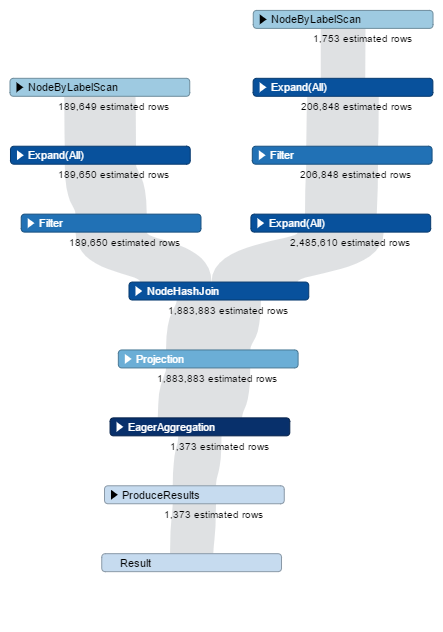
\includegraphics[scale=0.6]{pic/61.png}
\end{figure}

(2) match (u:User)-[]-(b:Badge)  match (u:User)-[]-(p:Post)  match (p:Post)-[]-(t:Tag)  return  t.TagName, id(u), id(b), id(p), count(*)

\begin {figure}[H]
\centering
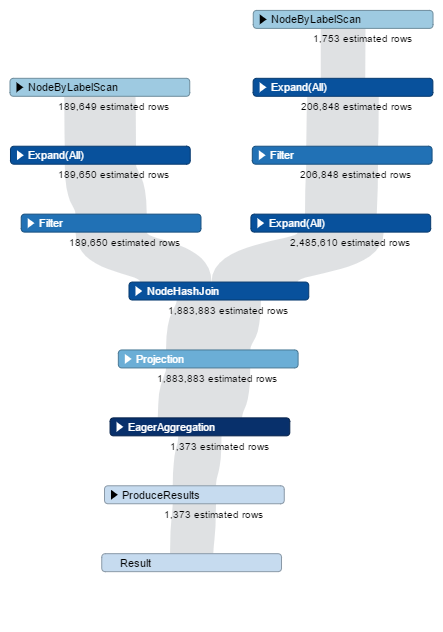
\includegraphics[scale=0.6]{pic/61.png}
\end{figure}

Since (2) contains ids of all queried nodes(User, Badge and Post), supposedly (2) should have a much larger result size than (1). However in Neo4j will estimate that (1) and (2) have the same result size. 

Therefore in our implementation we use the following function to predict cuboid size:
Cuiboid(att_1, att_2… att_n)= Product of(|att_i|) * (shrinking factor)^(n-1)
